%%%%%%%%%%%%%%%%%%%%%%%%%%%%%%%%%%%%%%%%%
%Final Year Project Report Bachelor of Engineering
% LaTeX Template

%Glasgow College, UESTC

%Arrangement Author: VAN DARKHOLME & Huang Yifan

%Email: 2288862h@student.gla.ac.uk 
%%%%%%%%%%%%%%%%%%%%%%%%%%%%%%%%%%%%%%%%%

%----------------------------------------------------------------------------------------
%	PACKAGES AND OTHER DOCUMENT CONFIGURATIONS
%----------------------------------------------------------------------------------------

\documentclass[
12pt, % The default document font size, options: 10pt, 11pt, 12pt
oneside, % Two side (alternating margins) for binding by default, uncomment to switch to one side
singlespacing, % Single line spacing, alternatives: onehalfspacing or doublespacing
parskip, % Uncomment to add space between paragraphs
]{article} % The class file specifying the document structure

\usepackage{geometry}

\usepackage[utf8]{inputenc} % Required for inputting international characters
\usepackage[T1]{fontenc} % Output font encoding for international characters
\usepackage{mathptmx}%%% Use the Times font by default%%%

\usepackage{color}%U can change font color

\usepackage[scaled]{helvet} % helvetica for sanserif, scaled 95% by default

\usepackage{courier}  % for typewriter text

\usepackage{textcomp} % lots of useful symbols

\usepackage{graphicx}  % inclusion of graphics files

\usepackage{hyperref}

\graphicspath{{Figures/}{./}}
%\addbibresource{bibliography.bib} % The filename of the bibliography
%----------------------------------------------------------------------------------------
%	THESIS INFORMATION (NECESSARY)
%----------------------------------------------------------------------------------------

\newcommand{\thesistitle}{Project Title} % Your thesis title, this is used in the , print it elsewhere with \thesistitle
\newcommand{\GUID}{11451419}% Your GUID, this is used in the , print it elsewhere with \GUID
\newcommand{\student}{Sajjad \textsc{Hussain}} % Your name, this is used in the title page and abstract, print it elsewhere with \student
\newcommand{\firstsupervisor}{\textcolor{red}{\tiny Keep blank before hardcopy submission}} % Your 1st supervisor's name, this is used in the title page, print it elsewhere with \firstsupervisor. YOU NEED TO KEEP BLANK FOR MOODLE SUBMISSION BUT PUT THE NAME BEFORE HARDCOPY SUBMISSION.
\newcommand{\secondsupervisor} {\textcolor{red}{\tiny Keep blank before hardcopy submission}}% Your 2nd supervisor's name, this is used in the title page, print it elsewhere with \secondsupervisor. YOU NEED TO KEEP BLANK FOR MOODLE SUBMISSION BUT PUT THE NAME BEFORE HARDCOPY SUBMISSION.

%----------------------------------------------------------------------------------------
%	OTHER INFORMATION 
%----------------------------------------------------------------------------------------

\newcommand{\degree}{Engineering} % Your degree name, this is used in the title page and abstract, print it elsewhere with \degree
\newcommand{\subject}{Electric & Electronic Engineering} % Your subject area, this is not currently used anywhere in the template, print it elsewhere with \subject
\newcommand{\keywords}{} % Keywords for your thesis, this is not currently used anywhere in the template, print it elsewhere with \keywords
\newcommand{\university}{\href{https://www.uestc.edu.cn/}{UETSC}} % Your university's name and URL, this is used in the title page and abstract, print it elsewhere with \university
\newcommand{\department}{\href{http://www.gla.uestc.edu.cn/}{Glasgow College}} % Your department's name and URL, this is used in the title page and abstract, print it elsewhere with \department


\newenvironment{declaration}{
	\newgeometry{left=4em,right=4em,bottom=6em,top=6em}
	\section*{Coursework Declaration and Feedback Form}
	\addcontentsline{toc}{section}{Coursework Declaration and Feedback Form}
	}{\clearpage\restoregeometry}

\renewenvironment{abstract}{
	\section*{Abstract}
	\bigskip
	\addcontentsline{toc}{section}{Abstract}}{\clearpage}

\newenvironment{acknowledgement}{
	\section*{Acknowledgements}
	\bigskip
	\addcontentsline{toc}{section}{Acknowledgements}}{\clearpage}


\geometry{
	paper=a4paper, % Change to letterpaper for US letter
	inner=6em, % Inner margin
	outer=6em, % Outer margin
	bindingoffset=0em, % Binding offset
	top=6em, % Top margin
	bottom=6em, % Bottom margin
	%showframe, % Uncomment to show how the type block is set on the page
}
\hypersetup{colorlinks=true,linkcolor=black,citecolor=black}% Remove read block in the content
\AtBeginDocument{
\hypersetup{pdftitle=\thesistitle} % Set the PDF's title to your title
\hypersetup{pdfauthor=\student} % Set the PDF's author to your name
\hypersetup{pdfkeywords=\keywords} % Set the PDF's keywords to your keywords
}



\begin{document}


\pagestyle{plain} % Default to the plain heading style until the thesis style is called for the body content

%----------------------------------------------------------------------------------------
%	TITLE PAGE
%----------------------------------------------------------------------------------------

\begin{titlepage}
\begin{center}


\includegraphics{Badge}
\vspace*{.08\textheight}

\textsc{\Large Final Year Project Report\\Bachelor of Engineering
}\\[2cm] % Thesis type

{\huge \bfseries \thesistitle\par}\vspace{3cm}% Thesis title

\begin{minipage}[t]{0.4\textwidth}
\begin{flushleft} \huge
Student:\\
\vspace*{.02\textheight}
GUID:\\
\vspace*{.02\textheight}
$1^{st}$\, Supervisor:\\
\vspace*{.02\textheight}
$2^{nd}$ Supervisor:\\
\end{flushleft}
\end{minipage}
\begin{minipage}[t]{0.4\textwidth}
\begin{flushright} \huge
\student\\
\vspace*{.02\textheight}
\GUID\\
\vspace*{.02\textheight}
\firstsupervisor\\
\vspace*{.02\textheight}
\secondsupervisor\\
\end{flushright}
\end{minipage}\\[3cm]

 
\vfill

{\huge 2019-2020}\\[2cm] % Date
%\includegraphics{Logo} % University/department logo - uncomment to place it
 
\end{center}
\end{titlepage}


\pagenumbering{roman}
%----------------------------------------------------------------------------------------
%	DECLARATION PAGE
%----------------------------------------------------------------------------------------
\renewcommand{\arraystretch}{1.3}
\begin{declaration}
\emph{This Student should complete and sign this part}
\\
\begin{table}[h!]
	\resizebox{\textwidth}{!}{
	\begin{tabular}{|p{6.5cm}|l|}
	\hline
	Student Name: \student & Student GUID: \GUID \\ \hline
	\begin{tabular}[c]{@{}l@{}}Course Code :\\ UESTC4006P\end{tabular} & \begin{tabular}[c]{@{}l@{}}Course Name :\\ INDIVIDUAL PROJECT 4\end{tabular} \\ \hline
	\begin{tabular}[c]{@{}l@{}}Name of 1st Supervisor:\\ \firstsupervisor \end{tabular} & \begin{tabular}[c]{@{}l@{}}Name of 2nd Supervisor:\\\secondsupervisor \end{tabular} \\ \hline
	\multicolumn{2}{|l|}{\begin{tabular}[c]{@{}l@{}}Title of Project:\\{\large\textbf{\thesistitle}} \end{tabular}} \\ \hline
	\multicolumn{2}{|l|}{\textbf{Declaration of Originality and Submission Information}} \\ \hline
	\textit{\begin{tabular}[c]{@{}l@{}}I affirm that this submission is all my\\own work in accordance with the \\University of Glasgow Regulations and \\the School of Engineering requirements \\Signed (Student) :\end{tabular}}
	&
	\multicolumn{1}{c|}{
\includegraphics[scale=0.5]{Figures/BarCode}}\\ \hline
	\multicolumn{2}{|l|}{Date of Submission :} \\ \hline
	\multicolumn{2}{|l|}{\textit{Feedback from Lecturer to Student – to be completed by Lecturer or Demonstrator}} \\ \hline
	\multicolumn{2}{|l|}{\begin{tabular}[c]{@{}l@{}}Grade Awarded:\\Feedback (as appropriate to the coursework which was assessed):\\ \\ \\ \\ \\ \\ \\ \\ \\\end{tabular}}\\ \hline
	\begin{tabular}[c]{@{}l@{}} Lecturer Demonstrator:\\ \\\end{tabular} & \begin{tabular}[c]{@{}l@{}}Date returned to the Teaching Office:\\ \\\end{tabular}\\ \hline
	\end{tabular}
	}
\end{table}

\end{declaration}
%----------------------------------------------------------------------------------------
%	ABSTRACT PAGE
%----------------------------------------------------------------------------------------

\begin{abstract}
All reports start with an \emph{abstract}, which contains a summary of the project: its aim, what was done and what was achieved. This document describes the requirements for a project report in the department and gives advice on how to get better marks. It is structured to match a project report as far as possible.
\end{abstract}

%----------------------------------------------------------------------------------------
%	ACKNOWLEDGEMENTS
%----------------------------------------------------------------------------------------

\begin{acknowledgement}
The acknowledgments and the people to thank go here, don't forget to include your project advisor
\end{acknowledgement}

%----------------------------------------------------------------------------------------
%	LIST OF CONTENTS
%----------------------------------------------------------------------------------------
\tableofcontents % Prints the main table of contents
\pagebreak
%----------------------------------------------------------------------------------------
%	THESIS CONTENT - SECTIONS
%----------------------------------------------------------------------------------------

\pagestyle{plain} % Return the page headers back to the "thesis" style

\pagenumbering{arabic}
% Include the sections of the thesis as separate files from the sections folder
% Uncomment the lines as you write the sections

\section{Introduction}

\emph{Whew -- I've finished the work, now I only have to write the report.} Sound familar? Many students put off writing until too late and don't leave enough time to make a good job of the report. This is a serious mistake because the report typically accounts for a large fraction of the assessment. Start early -- most people find report-writing difficult. Think about the report throughout your project, keep track of references and collect material to illustrate the report.

\subsection{Mechanical aspects}

The length of the body of the report will be specified in the instructions for the project. Extra material may be provided in appendices but this material should be for reference only: you cannot assume that the reader will study it. In other words, do not put vital points in an appendix.

You will probably think that the report is too short but this is deliberate. Most reports are submitted to busy managers, who do not have time to read lengthy documents. It is important to learn how to pick out the vital points and write a concise report with maximum impact.

Reports should be word-processed and firmly bound. Use A4 paper and a clear typeface such as 12-point Times, number the pages and leave margins of at least 25\,mm all round. Follow this layout (this document breaks some of the rules to keep it compact).
\begin{itemize}
\item
The front cover should show the title of the project with your name(s) and matriculation number(s) and the name of your supervisor(s).
\item
Put the abstract on the next page. It should be about 100--250 words and gives a brief summary of the report including the background and aims of the project, the principal results and conclusions.
\item
The next page should show the table of contents. 
\item
The body of the report should be divided into numbered sections, each starting on a new page. Figures (diagrams, plots or photographs) and tables need captions and should be numbered.
\end{itemize}

\subsection{What goes into the introduction?}

Explain the background to the project and the reasons why your particular piece of work was considered worthwhile. This leads to the \textbf{aims} of the project: what you are trying to achieve. Be specific. 
\section{Body of the report}

\subsection{Structure and sections}

The structure of the report and the titles of sections depend on the nature of the project. Here are suggestions for two extreme types, which can be adjusted to suit your report.

\subsubsection{Research projects}

Here you are given a starting point and a general direction: your aim is to discover something new. The report would probably be divided into sections with familiar titles.
\begin{itemize}
\item
\textbf{Theory} -- 
Explain essential background theory that is vital to understand your report. Select and present the material to show its relevance to the project and demonstrate your understanding. Do not repeat standard material from textbooks, which is a waste of space; give a reference instead. 
%Detailed mathematical derivations should be left to an appendix.

\item
\textbf{Experimental Techniques} --
Give an account of your experimental (or numerical) techniques. Emphasise details that would be necessary to continue the work or to compare your results with those of other experimenters. Aim to include what you would have liked to know at the start of your project.

\item
\textbf{Results} --
Describe these at an appropriate level of detail to support your conclusions. Lengthy tables should be left to an appendix or supplied on a CD. Avoid unnecessary detail: describe preliminary experiments briefly if at all, unless they illustrate some important point.
\end{itemize}


\subsubsection{Design, build and test projects}

Here the goal is specified, more or less precisely: your job is to work out how to get there. The titles of the sections are less standardised but here is a possible approach.
\begin{itemize}
\item
\textbf{Specification} --
Typically you are given only a vague description of the functions required and must first develop this into a firm specification against which your final product will be judged.
\item
\textbf{Possible strategies} --
Evaluate \emph{briefly} the possible approaches that you considered 
%for the overall design 
and explain why you selected one of these. 
Avoid excessive detail of discarded possibilities.
\item
\textbf{Implementation} --
Describe the final product. Concentrate on key features that required advanced design and skim over well-known aspects. Mention useful points that might help future students, such as tricky sections of data sheets.

\textbf{Software} is tricky. Often the best approach is to describe the high-level structure in the main text (a diagram of a state machine for example) and pick out any special features of the program. A complete listing should be included as an appendix or on a CD.
\item
\textbf{Testing} --
This is equivalent to the `Results' section of a research project. 
%and the same comments apply.
\end{itemize}


\subsection{Style of writing}

One of the most difficult aspects of writing is to judge the level and background of your readers. Typically the report will be assessed by your first supervisor, who is an expert on the topic, and your second supervisor, who is not. You should therefore assume that the reader is a \emph{well-educated, graduate engineer} but not an expert on the subject of the project. Assume that he or she is familiar with the general concepts taught in courses up to level 3 but not with the details of specialised courses at higher levels.

It is also difficult to appreciate that most readers are not interested in the nitty-gritty detail. They want to know \emph{what} you did and \emph{why} you did it that way but they don't want a step-by-step account of \emph{how} you did it. Your watchword should therefore be:
\begin{center}
\textbf{SUMMARISE!}
\end{center}
Of course some people need the details -- a person continuing work on the project requires precise experimental methods, for instance. Such material may be better in an appendix. The same is true for computer programs and schematics of complicated circuits. Design-and-build projects may need a User's Manual, which should be included as an appendix. 

A report is a formal document and should be written in appropriate language. Numerous books offer advice on writing reports and a selection \cite{jve05,mkm06,dfb09,tmy05} is listed in the references at the end. Here are a few tips.
\begin{itemize}
\item
Reports should be written in correct English. Break text into paragraphs, keep sentences to a reasonable length and insert appropriate punctuation. Use a spell-checker and a grammar-checker if desired but neither is a substitute for careful reading. 
\item
A report is not a story. 
%Write `The transistor exploded', not `I blew up the transistor'. Similarly, 
Write `The voltage was measured' rather than `I measured the voltage'. This document contains instructions and therefore uses a different style.
\item
Define all abbreviations when they are first used: `The accelerometer uses a serial peripheral interface (SPI)'. Provide a list of abbreviations if you use a large number of them.
\item
Don't write material that you don't understand. It will be obvious to the reader.
\end{itemize}
The quality of English is assessed as part of the report. Foreign students may feel this to be a burden but part of their education in this country is to learn to work effectively in an English-speaking environment. 

\subsection{Precision}

An engineering report must be precise. This applies both to the language and to numerical values. For example, the words \emph{precision} and \emph{accuracy} are often used interchangably in non-technical discussion but the distinction between them is vital in engineering.

Quote numerical results to an appropriate number of significant figures. For example, it is pointless to claim that a length was 12.345\,mm if it was measured with a pocket ruler. Don't simply write down all the digits displayed on your calculator. 

Analyse the uncertainties in your results to increase the impact of your results. Please avoid horrors like this:
\begin{quote}
The gain was quite accurate.
\end{quote}
The sentence is meaningless and the reader will doubt whether you have any idea of the accuracy. Contrast this sentence:
\begin{quote}
The accuracy of the gain was estimated to be $\pm 2\%$, limited by the tolerance of the resistors. A detailed analysis is given in Appendix C.
\end{quote}
This is informative and convinces the reader that you have a full understanding.

\subsection{Figures and tables}

\begin{figure}
\centering
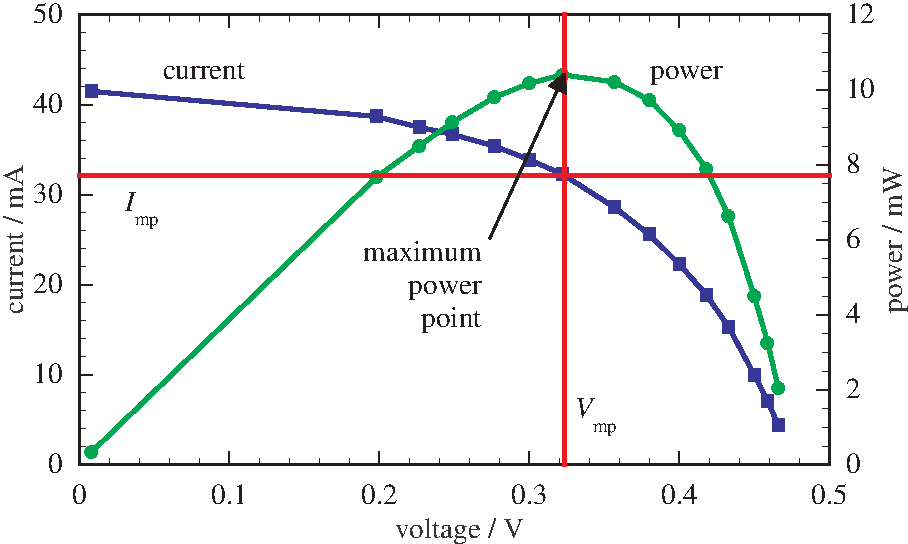
\includegraphics[scale=0.72]{solarcell}
\caption{Current and power as a function of voltage delivered by a single photovoltaic cell under illumination from a 150\,W metal halide floodlamp, showing the maximum power point.}
\label{solar cell fig}
\end{figure}

Figures and tables must have informative captions and be numbered as in Figure~\ref{solar cell fig}. Axes of graphs should have scales, titles and units, otherwise the plot is meaningless. All text must be legible, roughly the same size as the main text. Be warned that plots from Excel need extensive editing to bring them up to an acceptable standard. Oscilloscope screenshots can make good illustrations and are simple to capture on modern equipment.

Tables must have appropriate headings with units. Avoid lengthy tables: consider whether a graph would be clearer or the data would be better on a CD.

\subsection{References}

No project is done in isolation. A research project builds on the results of previous workers; a design-and-build project depends on the properties of the components available. You therefore draw on published documents during your project and must provide \emph{references} to these sources in your report. References are cited (a)~to give due credit to the originator and (b)~to guide a reader who wants more detailed information. You should give a reference wherever it is required for either of these purposes. Properly referenced material from many sources is a sign of a good project report. 
%This section explains how to present such references and how you will be penalised if you fail to do this. The mark for the report include an element for references to reflect their importance.

References must be cited with sequential numbers in square brackets where they are used in the text, not just listed at the end of the report. Typical usage is `Fitzmaurice and Hand \cite{gmf87} showed that\dots' or `The median is an appropriate estimator for this signal \cite{gmf87}'.

Avoid direct quotations from references in general; make it absolutely clear that the text is a quotation if this is unavoidable. An illustration, such as a diagram from a data sheet, is another type of quotation and must be referenced, typically in the figure caption. This is perfectly acceptable: do not waste time redrawing diagrams.

\subsubsection{Plagiarism}

If you copy from another person's work (project report, book, journal, web page or any other document) without acknowledging the source, you are guilty of \emph{plagiarism}. This is a disciplinary offence and the University has procedures for handling it. The failure to acknowledge a source is considered as plagiarism even if there was no deliberate intention to cheat. 

Avoid any risk of plagiarism by providing a reference for all sources that you use. Read the advice offered by the University Library and consult your supervisor if you are in any doubt. The University's \emph{Plagiarism Statement} is reproduced in Appendix \ref{plagiarism sect}.

\subsubsection{List of references}

All reports must have a section entitled `References' after the main text but before any appendices. This comprises a list of references, numbered to match the citations in the text. Each reference requires the following information and the cited references provide examples.
\begin{itemize}
\item
\textbf{Journal paper}: 
author(s), title of paper, name of journal, volume number, first page, last page and year \cite{gmf87}. 
Many journals now use article numbers instead of page numbers.
\item
\textbf{Book}: 
author(s), title, edition, publisher and year of publication \cite{jve05}.
Include the number of the chapter or page(s) if you refer to only a small part of the book.
\item
\textbf{Data sheet}: 
company, title, edition and date \cite{s08qg}. 
Application notes, technical reports and similar documents should be cited in the same way.
\item
\textbf{Web page}: 
author(s) or organisation, title, full URL and date of viewing \cite{mac09}. See below.
\end{itemize}
%The general rule is that 
The reader must be able to find the document without searching for further information.

\subsubsection{References from the Web}

The World Wide Web is a wonderful resource because it is so easy to search. It is therefore tempting to use web pages as references. \emph{Proceed with caution} because the accuracy of many web sites cannot be verified. This is particularly true for anonymous sites such as Wikipedia. Use them only as a starting point: good pages provide references to more authoritative sources.

Reports whose references are all or mainly from the web, especially from anonymous sites, will be penalised.
 
\include{Sections/Section3} 
\section{Conclusions}

Every report must have conclusions, built on the discussion. This section includes a summary of the main achievements of the work but is more than that. The noun `conclusion' can be defined as `a judgement or decision reached by reasoning' \cite{oupconc} so you should highlight what has been learnt as a result of your project. What is the big picture that the reader should take away? 

The Conclusions should include an assessment of the outcome against the original aims of the project. If you were unable to fulfil some aims, explain why. It is also useful to review the project plan (which should be included with the report). Did some tasks prove to be unexpectedly difficult, for instance?

\subsection{Suggestions for further work}

Almost every project leaves you with ideas for the future. Research typically answers some questions while opening new ones; by the end of a design-and-build project you may have thought of a superior approach. Examiners are impressed by intelligent suggestions for further work because they show that you really understand the project. It is often a sign of strength to identify the weak points and suggest solutions for them.


\clearpage % start appendices on a new page 
\begin{thebibliography}{9}
\addcontentsline{toc}{section}{References}
\bibitem{mkm06}
Marun K. Mitra,
\textit{Effective Technical Communication: A Guide for Scientists and Engineers},
Oxford
(2006).

\bibitem{dfb09}
David F. Beer and David McMurrey,
\textit{A Guide to Writing as an Engineer},
3rd Edition,
Wiley
(2009).

\bibitem{tmy05}
Trevor M. Young,
\textit{Technical Writing A--Z: A Commonsense Guide to Engineering Reports and Theses},
American Society of Mechanical Engineers
(2005).

\bibitem{gmf87}
G M Fitzmaurice and D J Hand, 
\textit{A comparison of two average conditional error estimators}, 
Pattern Recognition Letters, 
\textbf{6}, 
221--228 
(1987).

\bibitem{s08qg}
Freescale Semiconductor,
\textit{Datasheet for MC9S08QG microcontroller},
revision 4
(2008).

\bibitem{mac09}
Morgan Advanced Ceramics, 
\textit{Advanced Ceramics: Silicon Nitride}, \texttt{www.morgantechnicalceramics.com} 
(viewed 2009 May 13).

\bibitem{oupconc}
Oxford University Press, 
\textit{AskOxford},
\texttt{www.askoxford.com/?view=uk}
(viewed 2009 May 13).

`Conclusion' is defined as (1)~an end or finish, (2)~the summing-up of an argument or text, (3)~a judgement or decision reached by reasoning or (4)~the settling of a treaty or agreement.
\end{thebibliography}
\clearpage % start appendices on a new page
%----------------------------------------------------------------------------------------
%	THESIS CONTENT - APPENDICES
%----------------------------------------------------------------------------------------

\appendix % Cue to tell LaTeX that the following "chapters" are Appendices

% Include the appendices of the thesis as separate files from the Appendices folder
% Uncomment the lines as you write the Appendices

\section{Appendices}

Use appendices for supporting material which is relevant but of a detailed nature. In this way the flow of ideas in the body of the report is not interrupted. Appendices are usually lettered rather than numbered to distinguish them. Several uses for appendices have been suggested already but bear in mind that a CD may be more appropriate for large tables of results, long programs and data sheets or other background information. Appendices are not included in the word count because the assessors are not obliged to read them. Do not put vital points here!

Include your project plan and interim reports as appendices on paper.

\section{University's Plagiarism Statement}
\label{plagiarism sect}

The University's degrees and other academic awards are given in recognition of a student's personal achievement. All work submitted by students for assessment is accepted on the understanding that it is the student's own effort. 

Plagiarism is defined as the submission or presentation of work, in any form, which is not one's own, without acknowledgement of the sources. Plagiarism includes inappropriate collaboration with others. Special cases of plagiarism can arise from a student using his or her own previous work (termed auto-plagiarism or self-plagiarism). Autoplagiarism includes using work that has already been submitted for assessment at this University or for any other academic award.

The incorporation of material without formal and proper acknowledgement (even with no deliberate intent to cheat) can constitute plagiarism. Work may be considered to be plagiarised if it consists of: 
\begin{itemize}
\item
a direct quotation; 
\item
a close paraphrase; 
\item
an unacknowledged summary of a source; 
\item
direct copying or transcription.
\end{itemize}
With regard to essays, reports and dissertations, the rule is: if information or ideas are obtained from any source, that source must be acknowledged according to the appropriate convention in that discipline; and any direct quotation must be placed in quotation marks and the source cited immediately. Any failure to acknowledge adequately or to cite properly other sources in submitted work is plagiarism. Under examination conditions, material learnt by rote or close paraphrase will be expected to follow the usual rules of reference citation otherwise it will be considered as plagiarism. Departments should provide guidance on other appropriate use of references in examination conditions. 

Plagiarism is considered to be an act of fraudulence and an offence against University discipline. Alleged plagiarism, at whatever stage of a student's studies, whether before or after graduation, will be investigated and dealt with appropriately by the University.

The University reserves the right to use plagiarism detection systems, which may be externally based, in the interests of improving academic standards when assessing student work.


%----------------------------------------------------------------------------------------
%	BIBLIOGRAPHY
%----------------------------------------------------------------------------------------

%\printbibliography[heading=bibintoc]

%----------------------------------------------------------------------------------------

\end{document}  
